\subsection{Effect of different window sizes for dense SIFT}
\begin{figure}[H]
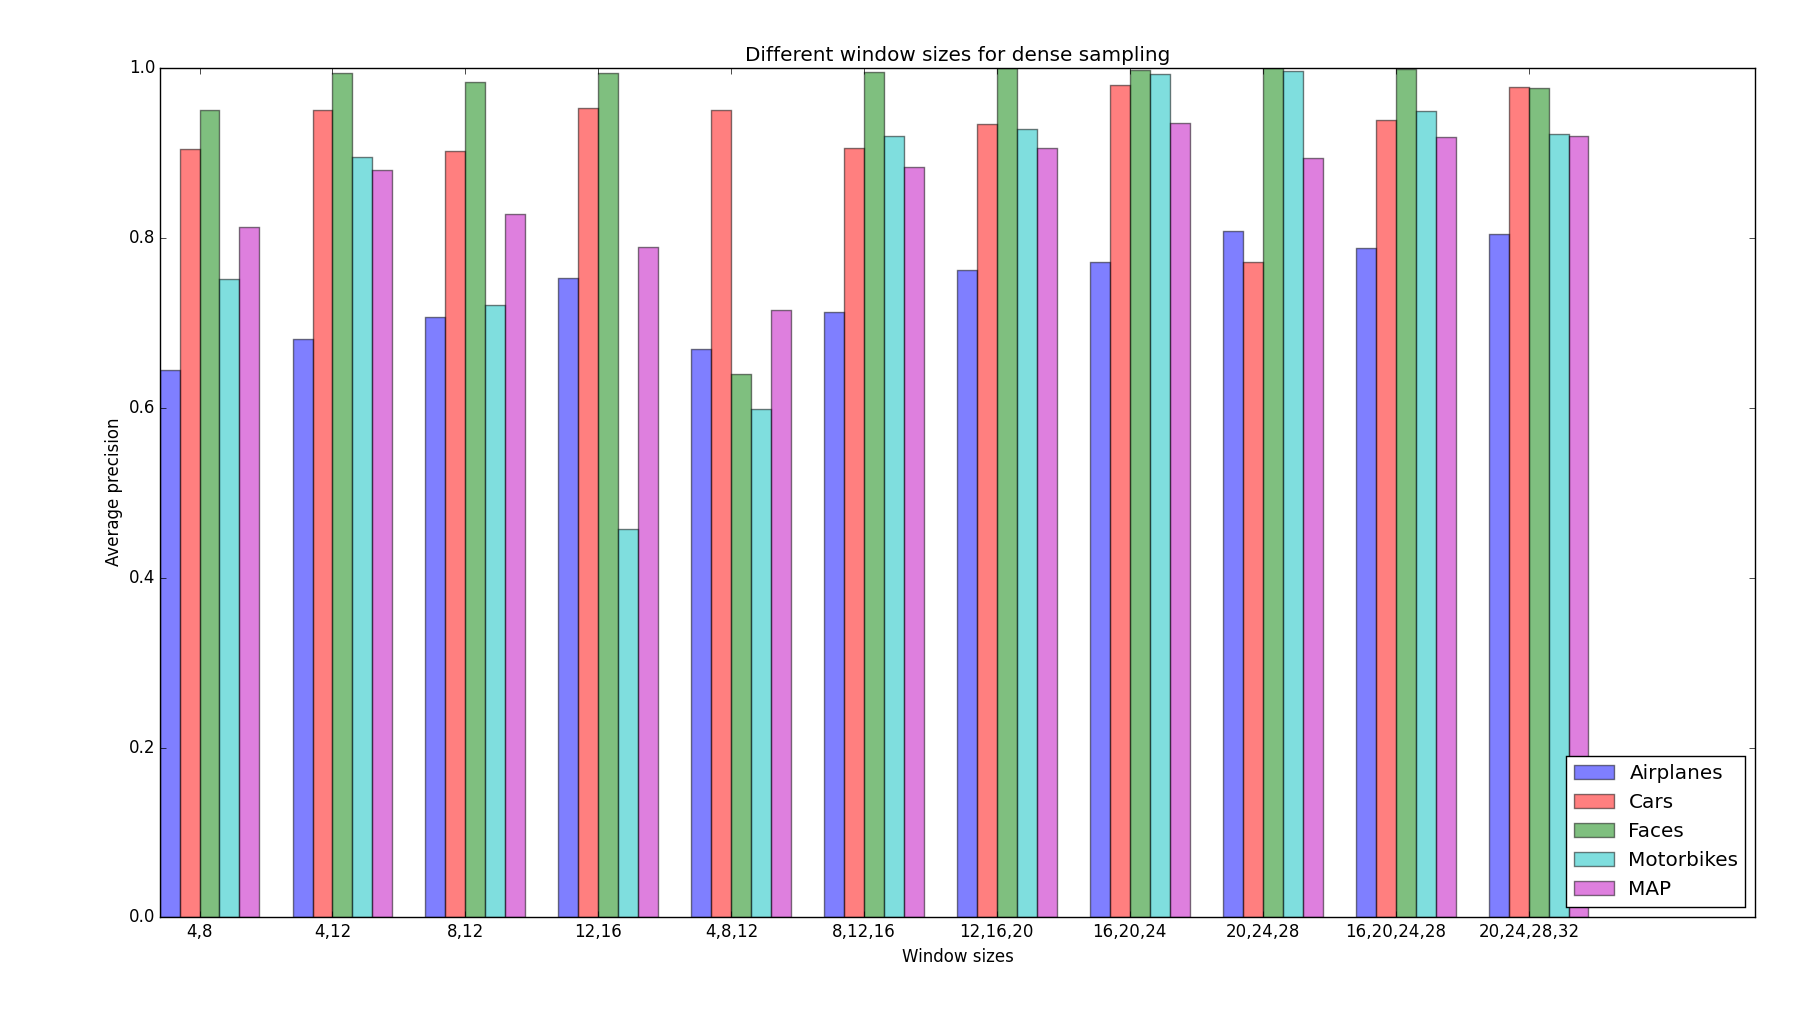
\includegraphics[width=\textwidth]{../plots/window_sizes_dense}
\caption{Effect of different window sizes on dense SIFT}
\end{figure}
\begin{table}[H]
\begin{tabular}{|c|ccccc|}
\hline
\textbf{Window size} & \textbf{AP Airplanes} & \textbf{AP Cars} & \textbf{AP Faces} & \textbf{AP Motorbikes} & \textbf{MAP}\\
\hline
4, 8 & 0.6447 & 0.9053 & 0.9510 & 0.7516 & 0.8132\\
4, 12 & 0.6809 & 0.9505 & 0.9945 & 0.8955 & 0.8803\\
8, 12 & 0.7066 & 0.9031 & 0.9839 & 0.7216 & 0.8288\\
12, 16 & 0.7532 & 0.9529 & 0.9939 & 0.4570 & 0.7893\\
4, 8, 12 & 0.6698 & 0.9511 & 0.6400 &  0.5987 & 0.7149\\
8, 12, 16 & 0.7133 & 0.9064 & 0.9952 & 0.9199 & 0.8837 \\
12, 16, 20 & 0.7629 & 0.9349 & 1.0000 & 0.9280 & 0.9065 \\
16, 20, 24 & 0.7719 & 0.9803 & 0.9981 & 0.9927 & 0.9357 \\
20, 24, 28 & 0.8086 & 0.7713 & 1.0000 & 0.9965 & 0.8941 \\
20, 24, 28, 32 & 0.8042 & 0.9782 & 0.9770 & 0.9223 & 0.9204 \\
16, 20, 24, 28 & 0.7882 & 0.9395 & 0.9989 & 0.9501 & 0.9192 \\

\hline
\end{tabular}
\caption{Effect of different window sizes for dense SIFT,  Color space: opponent}
\label{tab:winsize}
\end{table}

The effect of changing the window size for dense SIFT sampling is shown in table \ref{tab:winsize}. The best results are achieved by having a range of window sizes, since this captures a range of feature from details to larger features. However, a wider range of window sizes does not result in a better performance, since this captures too many features, the data tends to overfit. Smaller window sizes, even in a range, also underperform since these ranges are not capable of capturing larger features, like wings of airplanes and entire cars. 